%%%%%%%%%%%%%%%%%%%%%%%%%%% asme2e.tex %%%%%%%%%%%%%%%%%%%%%%%%%%%%%%%
% Template for producing ASME-format articles using LaTeX            %
% Written by   Harry H. Cheng                                        %
%              Integration Engineering Laboratory                    %
%              Department of Mechanical and Aeronautical Engineering %
%              University of California                              %
%              Davis, CA 95616                                       %
%              Tel: (530) 752-5020 (office)                          %
%                   (530) 752-1028 (lab)                             %
%              Fax: (530) 752-4158                                   %
%              Email: hhcheng@ucdavis.edu                            %
%              WWW:   http://iel.ucdavis.edu/people/cheng.html       %
%              May 7, 1994                                           %
% Modified: February 16, 2001 by Harry H. Cheng                      %
% Modified: January  01, 2003 by Geoffrey R. Shiflett                %
% Use at your own risk, send complaints to /dev/null                 %
%%%%%%%%%%%%%%%%%%%%%%%%%%%%%%%%%%%%%%%%%%%%%%%%%%%%%%%%%%%%%%%%%%%%%%

%%% use twocolumn and 10pt options with the asme2e format
\documentclass[cleanfoot,cleanhead,onecolumn,10pt,notitlepage]{asme2e}
\special{papersize=8.5in,11in}

\usepackage{listings}
\usepackage{graphicx}
\usepackage{amsmath}
\usepackage[hidelinks]{hyperref}
\lstset{
    breaklines=true, % break lines for files
    basicstyle=\scriptsize,
    numbers=left,
    showstringspaces=false,
    frame=l
}

%% The class has several options
%  onecolumn/twocolumn - format for one or two columns per page
%  10pt/11pt/12pt - use 10, 11, or 12 point font
%  oneside/twoside - format for oneside/twosided printing
%  final/draft - format for final/draft copy
%  cleanfoot - take out copyright info in footer leave page number
%  cleanhead - take out the conference banner on the title page
%  titlepage/notitlepage - put in titlepage or leave out titlepage
%  
%% The default is oneside, onecolumn, 10pt, final

%%% You need to remove 'DRAFT: ' in the title for the final submitted version.
\title{Major Project \# 1}

%%% first author
\author{Shaun Harris
    \affiliation{
	Department of Mechanical and Aerospace Engineering\\
	Utah State University \\
    Email: shaun.r.harris@gmail.com
    }
}


\begin{document}

\maketitle    

%%%%%%%%%%%%%%%%%%%%%%%%%%%%%%%%%%%%%%%%%%%%%%%%%%%%%%%%%%%%%%%%%%%%%%

\begin{abstract}
    {\it A transfer orbit from Low Earth Orbit to Medium Earth Orbit is investigated.  Four separate maneuvers are investigated and compared.  The numerical algorithm used is also presented and described.}
\end{abstract}


\tableofcontents

%%%%%%%%%%%%%%%%%%%%%%%%%%%%%%%%%%%%%%%%%%%%%%%%%%%%%%%%%%%%%%%%%%%%%%

\begin{nomenclature}
\entry{$a_{LEO}$}{Radius of Low Earth Orbit $\approx 8530km$}
\entry{$a_{MEO}$}{Radius of Medium Earth Orbit $\approx 13200km$}
\entry{$\bar{X}$}{Matrix containing $r, \nu, V_r, V_v,$ and $m$}
\entry{$r$}{Location in the $r$-direction}
\entry{$\nu$}{Location in the $\nu$-direction}
\entry{$V_r$}{Velocity in the $r$-direction}
\entry{$V_\nu$}{Velocity in the $\nu$-direction}
\entry{$m$}{Mass of satellite}
\entry{$m_{propellant}$}{Mass of propellant used to get into final orbit}
\entry{$\left.m_{propellant}\right|_1$}{Amount of propellant used at first thrust}
\entry{$\left.m_{propellant}\right|_2$}{Amount of propellant used at second thrust}
\entry{$\Delta V_1$}{Change in velocity for first thrust to get into transfer orbit}
\entry{$\Delta V_2$}{Change in velocity for second thrust to get into circular final orbit}
\entry{$\Delta V_{tot}$}{Change in velocity for combined thrust to get into circular final orbit}
\entry{$dt$}{Time interval for numerical algorithm}
\end{nomenclature}

%%%%%%%%%%%%%%%%%%%%%%%%%%%%%%%%%%%%%%%%%%%%%%%%%%%%%%%%%%%%%%%%%%%%%%

\section{INTRODUCTION}

There were four sections to this problem statement.  The overall goal was achieve a simulation that would produce a satellite's trajectory moving from $a_{LEO}$ to $a_{MEO}$. A Homann Transfer calculation was used to compare to this trajectory.  The following two equations (Eq. \ref{eq:low} and \ref{eq:high})

\begin{equation}
\begin{aligned}
F_{thrust} &= 10 N \\
I_{sp} &= 2000 s
\label{eq:low}
\end{aligned}
\end{equation}

\begin{equation}
\begin{aligned}
F_{thrust} &= 2000 N \\
I_{sp} &= 270 s
\label{eq:high}
\end{aligned}
\end{equation}

\subsection{Part a}

The parameters in Eq. \ref{eq:low} are for the low thrust burn.  This burn is used first to get into the transfer orbit.  Once the transfer orbit is reached, we then coast until at the apogee and then use an impulsive calculation using the parameters in Eq. \ref{eq:high} to get into the circular orbit in $a_{MEO}$.  

Additionally, both a trapezoidal rule and the Runge-Kutta integration schemes were applied.  The time interval was then altered to see where the algorithm blows up.

The resulting $\Delta V$ and $m_{propellant}$ were then compared to other parts of this problem.

\subsection{Part b}

This is similar to part a, except that both maneuvers were performed impulsively the parameters in Eq. \ref{eq:high} was used both times.  This was exactly the Homann Transfer calculation using the impulsive motor.  We calculated the $\Delta V$ and $m_{propellant}$ and compared these results to part a.


\subsection{Part c}

This analysis a complete continuous large thrust transfer.  Meaning both the first and second thrust was calculated using a continuous motor.  Eq. \ref{eq:high} describes the parameters for the motor used.  It was shown that the $dt$ value was required to be fairly small in order for the numerical algorithm to accurately predict the satellite's position.

\subsection{Part d}

This part of the problem statement did not require much change from the calculations in part c.  The only change was the time that the second thrust began.  This was done by manually altering the time that the coasting section ended the second thrust began.  It was aimed so that the total $\Delta V_2$ was centered around the when the orbit would reach the required apogee if it was coasting.  


%%%%%%%%%%%%%%%%%%%%%%%%%%%%%%%%%%%%%%%%%%%%%%%%%%%%%%%%%%%%%%%%%%%%%%

\section{NUMERICAL ALGORITHM}

In order to program this prediction method, several numerical algorithms were used.  A matrix of values describing the orbit and satellite location was created.  This was titled $\bar{X}$.  The values it contained is shown in Eq. \ref{eq:X}.  

\begin{equation}
\begin{aligned}
\bar{X} &= \left[r, \nu, V_r, V_\nu, m\right]
\label{eq:X}
\end{aligned}
\end{equation}

This matrix had several equations that was know in order to calculate the time derivative of $\bar{X}$.  These equations were used along with the Trapezoidal and Runge-Kutta numerical integration scheme.  These schemes provided the next step in the satellite's orbit.  The four phases of the orbit were then used in parallel with these integration schemes to yield the orbit transfer for each of the parts of the problem stated above.  

The trapezoidal algorithm was analyzed in part a.  When the $dt$ value was steadily increased we could see the performance of the algorithm.  The steps between each point on the plot got larger, and the values got less accurate.  It was found that at high $dt$ the trajectory was not calculated correctly.  Fig. \ref{fig:aa} shows the resulting trajectory.  It can be seen that if the $dt = 500$ we find that the coasting process seems to enter an escape velocity.  This is impossible and we instantly know that the numerical algorithm has failed to calculate the correct result for each step.

The code in Appendix \ref{sec:code} shows the program created to solve this problem.  

\section{RESULTS}

Four separate transfer orbits were described and will be analyzed below.

\subsection{Part a}

The resultant trajectory is shown in Fig. \ref{fig:aa}.  The large $dt$ value was previously described, but when the code did have a small enough $dt$ value we found the results shown here.

$\Delta V_1 = 1321.034$

$\Delta V_2 = 19.499$

$\Delta V_{tot} = 1340.533$

$m_{propellant} \approx 77.6$ 

We can see here that the rocket equation does not accurately depict what is happening.  This can be seen by comparing these values to the values calculated by the rocket equation in part b.  Note that the $\Delta V_1$ and $\Delta V_2$ values are off.  But the $\Delta V_{tot}$ is fairly accurate still.
 


\subsection{Part b}

Doing the Homann Transfer calculations yielded the results shown here.

$\Delta V_1 = 698.829$

$\Delta V_2 = 626.159$

$\Delta V_{tot} = 1324.988$

$m_{propellent} \approx 393.739$

Comparing these results to Part a we find that the impulsive Homann Transfer used more mass propellent, but required less $\Delta V_{tot}$.  Thus the Homann Transfer was a more efficient transfer orbit, but the motor used in part a required less mass to achieve the same orbit transfer.  No figure is shown here since the equations did not require any numerical algorithm.  They only required the used of the Homann Transfer equations.

\subsection{Part c}

Doing this transfer and the calculations provided the results shown here.

$\Delta V_1 = 705.611$

$\Delta V_2 = 774.191$

$\Delta V_{tot} = 1479.802$

$m_{propellent} \approx 745.531$

The trajectory is shown in Fig. \ref{fig:cd}.  We can see here that the trajectory is reached sooner, but it costs more propellant in order to reach the same orbit.  


\subsection{Part d}

Doing this transfer and the calculations provided the results shown here.

$\Delta V_1 = 701.576$

$\Delta V_2 = 627.3218$

$\Delta V_{tot} = 1328.8978$

$m_{propellent} \approx 688.01414$

$\left.m_{propellant}\right|_1 = 406.3272$

$\left.m_{propellant}\right|_2 = 281.68694$

The trajectory is shown in Fig. \ref{fig:cd}.  We can see here that the trajectory is similar to part c, but that it took a little less propellant to reach the orbit.  Obviously, it is more efficient to begin the final boost before the apogee is reached.


%%%%%%%%%%%%%%%%%%%%%%%%%%%%%%%%%%%%%%%%%%%%%%%%%%%%%%%%%%%%%%%%%%%%%%

\section{CONCLUSION}

The most efficient orbit, in terms of $m_{propellant}$ was part a.  This transfer took the least amount of propellant overall.  Though, it should be noted that it did take a significantly longer time to reach the orbit.  If time was of importance, than another orbit may have been desired.  Likely, the orbit transfer in part d would be the most realistic choice if speed was of importance. 

Ideally part b would be the fastest transfer in orbit.  But it takes an unrealistic impulse in speed to accommodate the transfer.  This Homann Transfer in part b is a fairly accurate approximation of the true $\Delta V$ values.   It should be noted though that the rocket equations are inaccurate when applied to a long duration non-impulsive burn such as in part a.  We can see that the rocket equations do not accurately depict what is happening.  

%%%%%%%%%%%%%%%%%%%%%%%%%%%%%%%%%%%%%%%%%%%%%%%%%%%%%%%%%%%%%%%%%%%%%%

%\bibliographystyle{asmems4}
%\bibliography{asme2e}

%%%%%%%%%%%%%%%%%%%%%%%%%%%%%%%%%%%%%%%%%%%%%%%%%%%%%%%%%%%%%%%%%%%%%%

%\section*{FIGURES}

\begin{figure}[t]
\begin{center}
    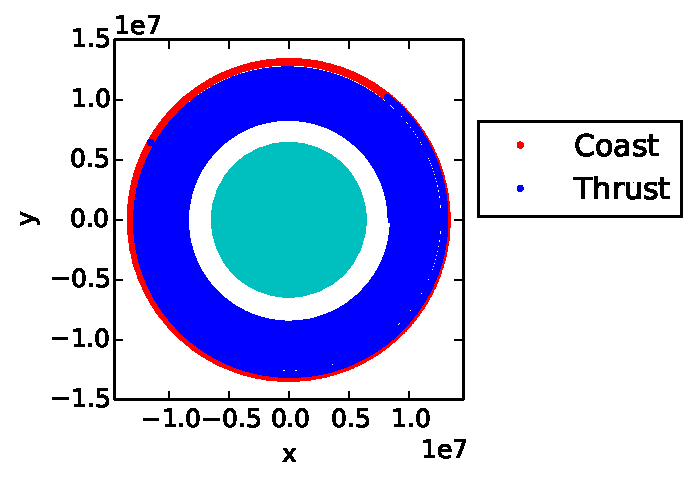
\includegraphics[width=0.45\linewidth]{../python_stuff/part_a.pdf}
    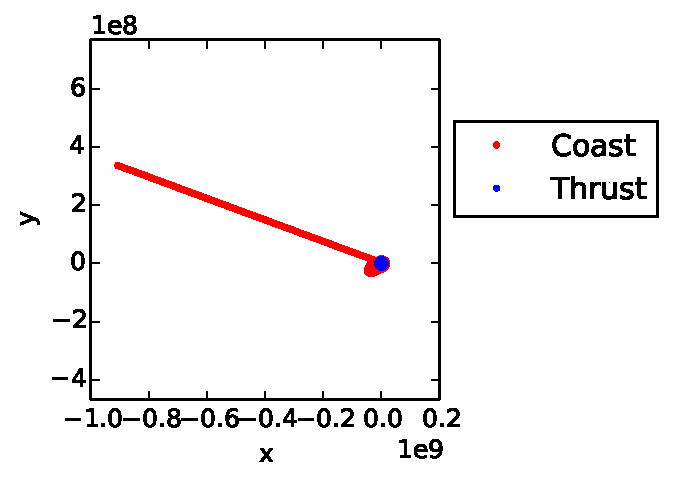
\includegraphics[width=0.45\linewidth]{../python_stuff/part_a_blowup.pdf}
    \caption{\textbf{Left:}Plot of trajectory for part a.  \textbf{Right:}  Plot of trajectory for part a when the $dt = 500$.}
    \label{fig:aa}
\end{center}
\end{figure}

\begin{figure}[t]
\begin{center}
    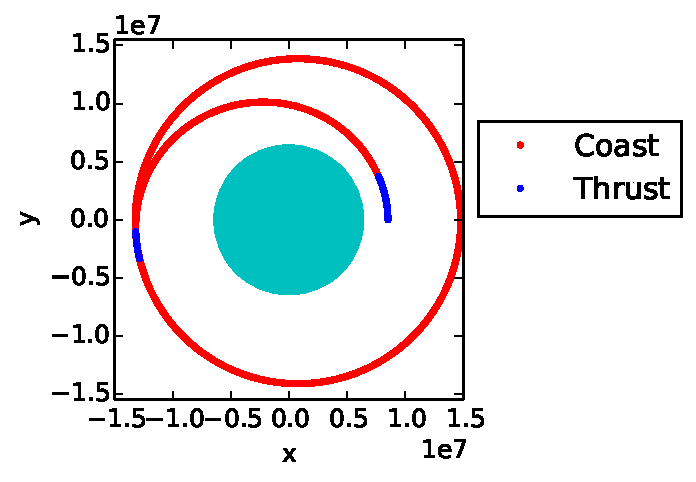
\includegraphics[width=0.45\linewidth]{../python_stuff/part_c.pdf}
    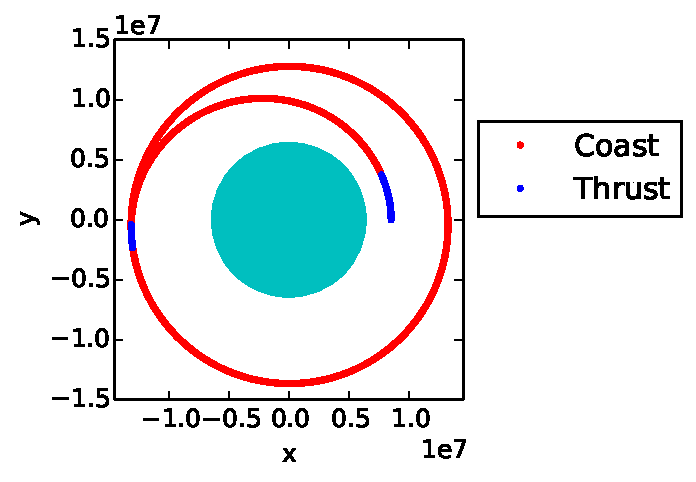
\includegraphics[width=0.45\linewidth]{../python_stuff/part_d.pdf}
    
    \caption{\textbf{Left: }Plot of trajectory for part c.  \textbf{Right: }Plot of trajectory for part d.}
    \label{fig:cd}
\end{center}
\end{figure}

%%%%%%%%%%%%%%%%%%%%%%%%%%%%%%%%%%%%%%%%%%%%%%%%%%%%%%%%%%%%%%%%%%%%%%
%\clearpage

\appendix

\section{Appendix A: Code}
\label{sec:code}
\subsection*{Header files}
\lstinputlisting[language=c++]{../cpp_stuff/DEFS.h}
\lstinputlisting[language=c++]{../cpp_stuff/X.h}
\subsection*{Linked c\texttt{++} file}
\lstinputlisting[language=c++]{../cpp_stuff/X.cpp}
\subsection*{Main Program}
\lstinputlisting[language=c++]{../cpp_stuff/Project1.cpp}





\end{document}
